\documentclass[11pt,letterpaper]{article}

% include figures
\usepackage{graphicx}
% get nice colors
\usepackage{xcolor}

% change default font to Palatino (looks nicer!)
\usepackage[latin1]{inputenc}
\usepackage{mathpazo}
\usepackage[T1]{fontenc}
% load some useful math symbols/fonts
\usepackage{latexsym,amsfonts,amsmath,amssymb,wasysym}
% be able to insert code
\usepackage{listings}

% comfort package to easily set margins
\usepackage[top=1in, bottom=1in, left=1in, right=1in]{geometry}

% spacing after a paragraph
\setlength{\parskip}{.15cm}
% indentation at the top of a new paragraph
\setlength{\parindent}{0.0cm}
% make units not slanted in math mode
\newcommand{\unit}[1]{\ensuremath{\, \mathrm{#1}}}

\begin{document}

\begin{center}
\Large
Ay190 -- Worksheet 10\\
Daniel DeFelippis\\
Date: \today
\end{center}

%%
%%
%% I worked with Scott Barenfeld
%%
%% All python code can be found in the ws10 directory in my repository
%%
%%

\section*{Solution of a simple BVP}

We are solving
\begin{align*}
\frac{dy}{dx} &= u(x), \\
\frac{du}{dx} &= 12x - 4, \\
y(0) &= 0, \hspace{4pt} y(1) = 0.1. 
\end{align*}
using both Euler and RK2 integrators.

Implementing both for 10, 50, 200, and 1000 points, we find that all the 
Euler integrator only needs two iterations for the error to go below the 
threshold of $10^{-12}$, even with the outlandish choices of $z_0$ and $z_1$, for
all of the different numbers of points. The RK2 integrator only needs one! 
Below are the final values of $z$ calculated by the integrators.
\begin{center}
    \begin{tabular}{| l | l | l | l | l |}
    \hline
    npoints & $z_{final}$ (Euler) & $z_{final}$ (RK2) \\ \hline
    10 & 0.495061728395  & 0.124691357836 \\ \hline
    50 & 0.17996668055 & 0.100832985714 \\ \hline
    200 & 0.119999494962 & 0.100050503388 \\ \hline
    1000 & 0.103999995992 & 0.100002001971 \\
    \hline
    \end{tabular}
\end{center} 

The values of $z$ seem to be converging to z = 0.1 for large numbers of points.
It should do this because the actual solution to the BVP is 
$$y = 2x^3 - 2x^2 + 0.1x, $$
which means $z = y'(0) = 0.1$. 

To demonstrate convergence, we look at 
$$ Q = \frac{|y(x; h_2) - y(x)|}{|y(x; h_1) - y(x)|} = \left(\frac{h_2}{h_1}\right)^n $$
where $y(x)$ is the actual solution, and $h_1$ and $h_2$ are step sizes with $h_1 > h_2$. 
Choosing the step sizes $h_1 = 1/(10-1) = 1/9$ and $h_2 = 1/(1000-1) = 1/999$, we get that
$Q = (1/111)^n \approx (0.009)^n$, where $n$ is the order of convergence. 

For the Euler Integrator, we get that $Q = 0.00912161248173$ (using the maximum
differences between the calculated and actual solutions in the formula), which clearly
indicates that the order of convergence is $n = 1$ as we expect. 

For the RK2 integrator, we get the strange value $Q = 10.792093469$. To see why this is 
happening, we examine the plots of the two integrators with the actual solution. 

\newpage

\begin{figure}[bth]
\centering
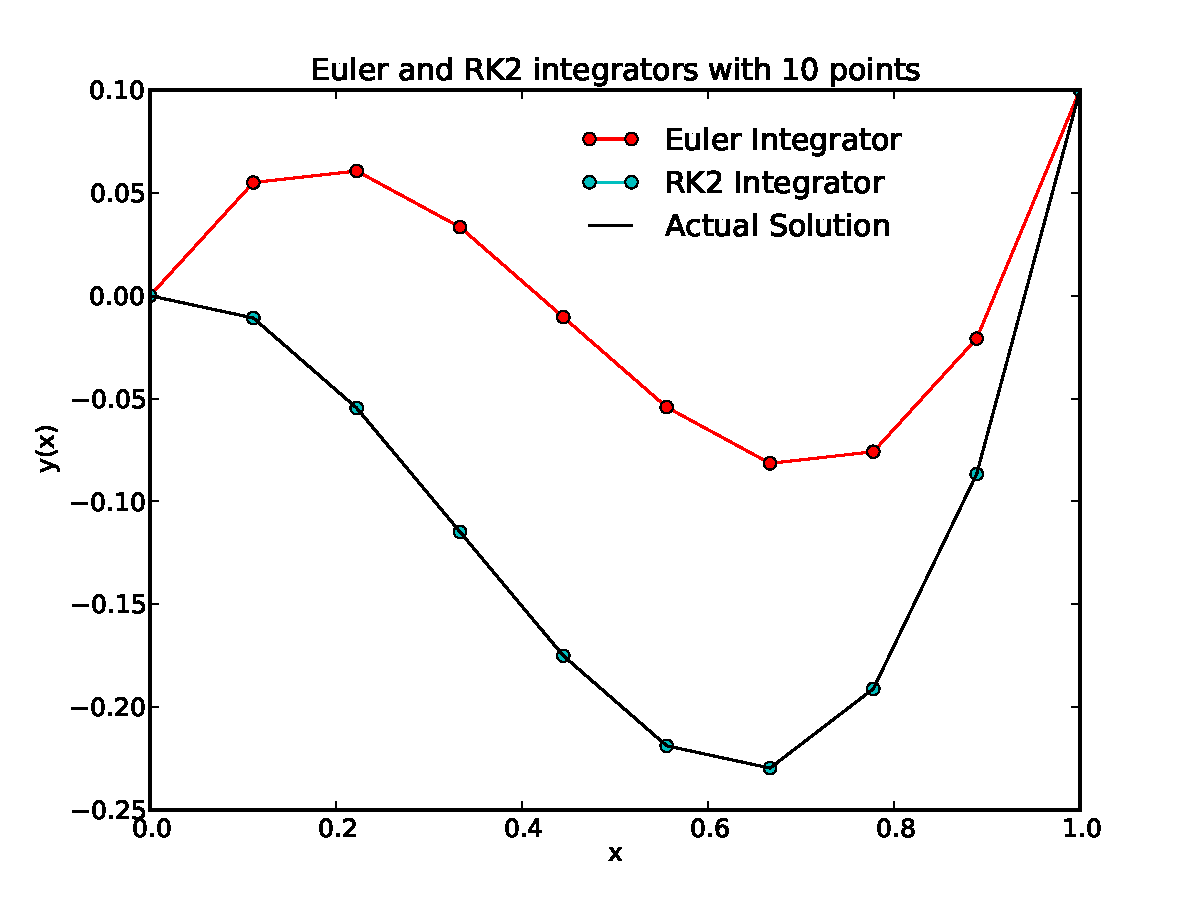
\includegraphics[width=0.61\textwidth]{10points.pdf}
\caption{Euler and RK2 integrators with 10 points}
\label{fig:10points}
\end{figure}

\begin{figure}[bth]
\centering
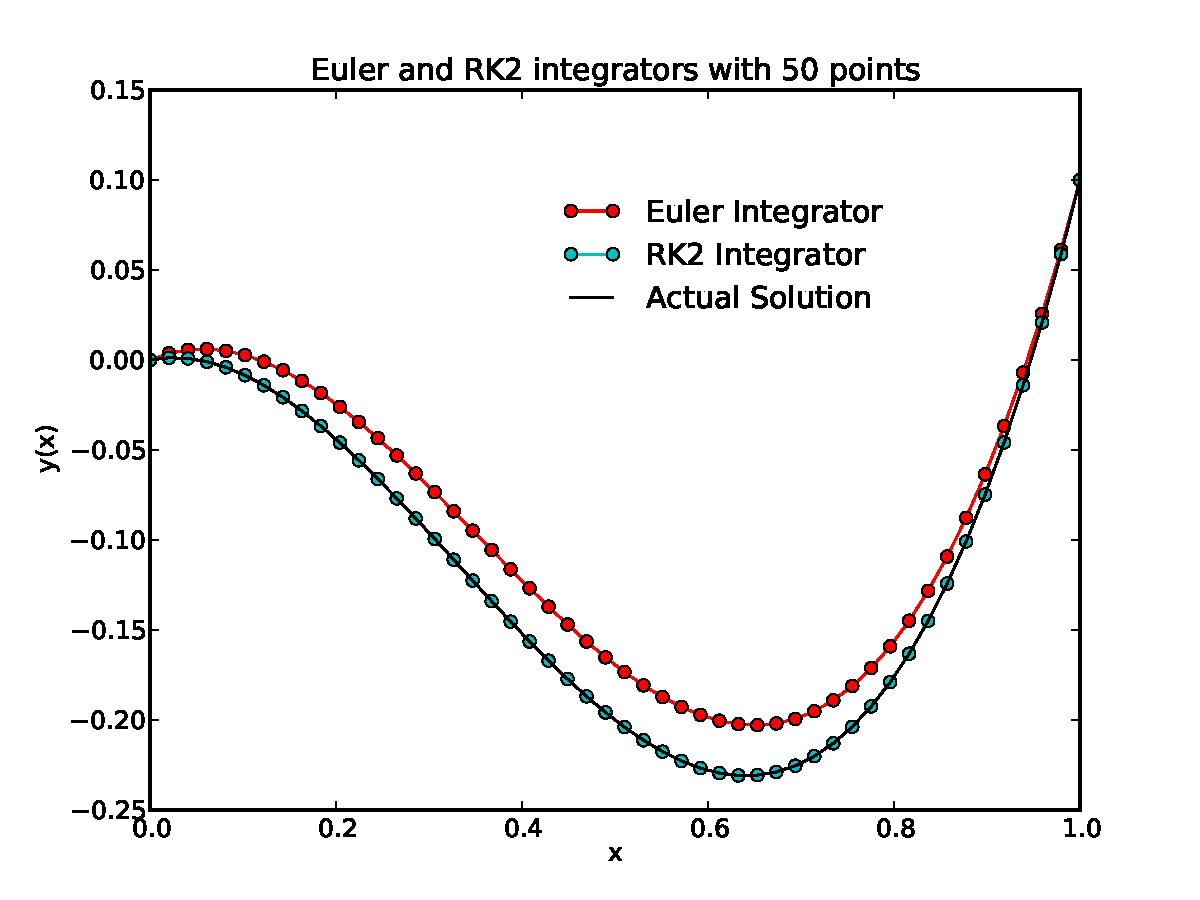
\includegraphics[width=0.61\textwidth]{50points.pdf}
\caption{Euler and RK2 integrators with 50 points}
\label{fig:50points}
\end{figure}

\begin{figure}[bth]
\centering
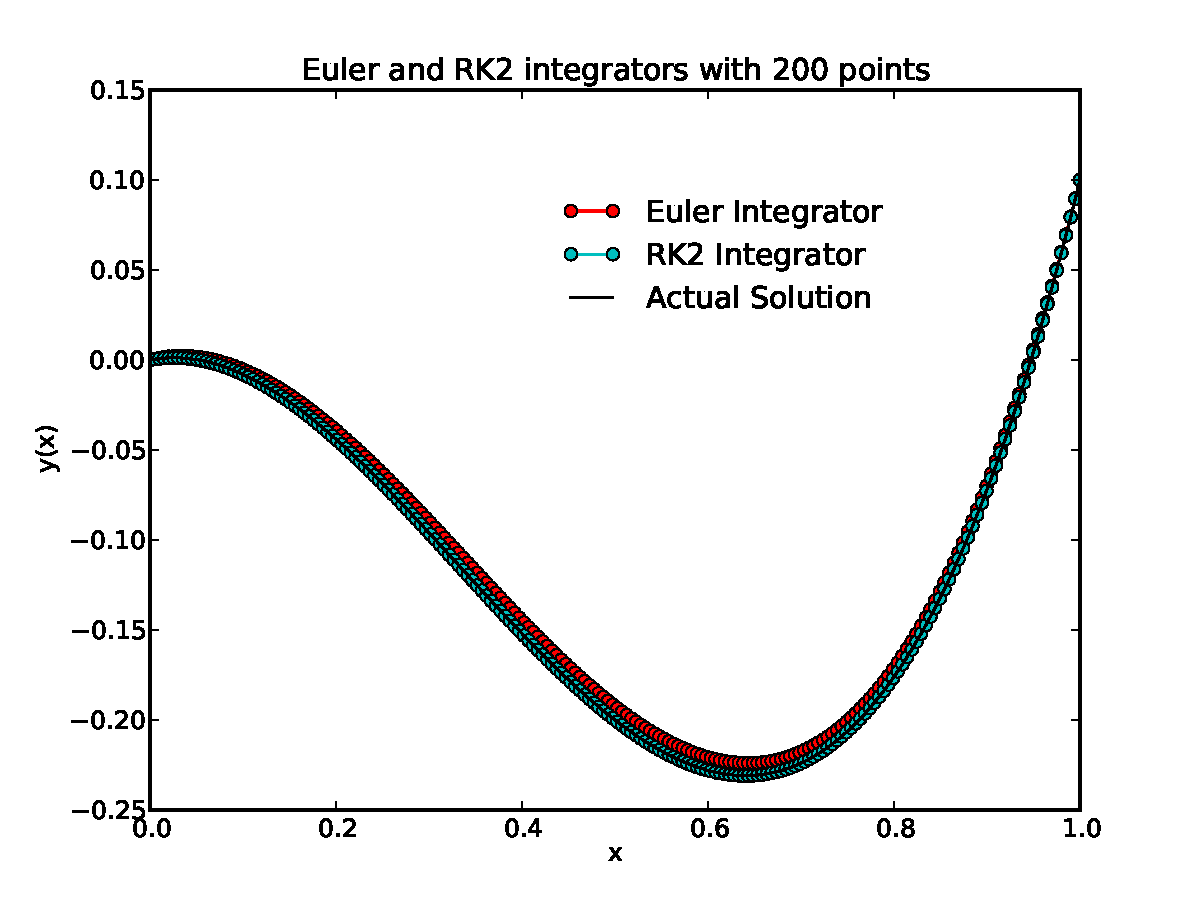
\includegraphics[width=0.75\textwidth]{200points.pdf}
\caption{Euler and RK2 integrators with 200 points}
\label{fig:200points}
\end{figure}

\begin{figure}[bth]
\centering
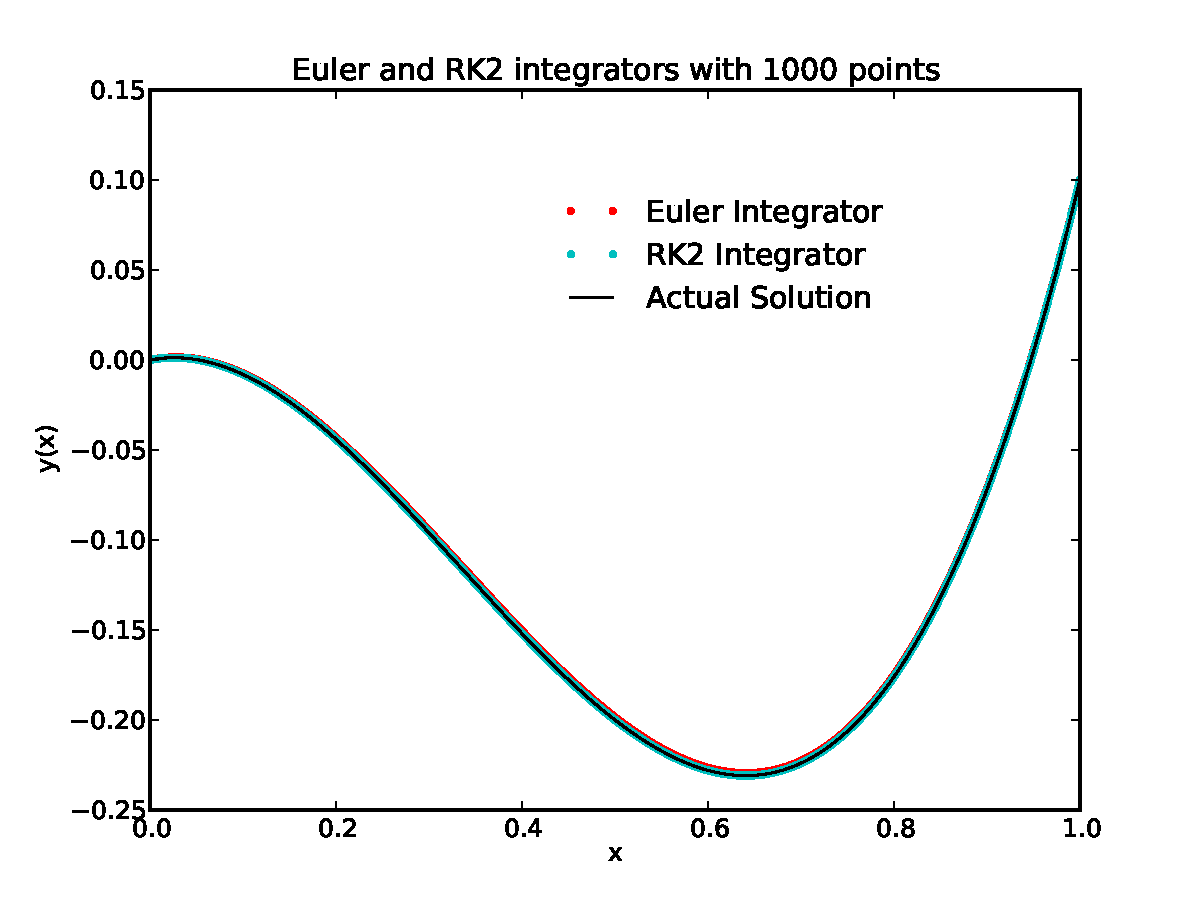
\includegraphics[width=0.75\textwidth]{1000points.pdf}
\caption{Euler and RK2 integrators with 1000 points}
\label{fig:1000points}
\end{figure}

We see that the RK2 integrator, even for the relatively small value of 10 points,
seems to plot the actual solution exactly! Therefore, it makes sense that the Q factor
is so weird because we are dividing by essentially 0. To explain why this happens, we note 
that the error in the RK2 integrator contains order $h^3$ terms and higher, which
correspond to the third derivative of $u(x)$ in the equation 
$$ \frac{dy}{dx} = u(x). $$
That is, when we expand $u(x)$, the lowest order error term for the RK2 method is 
$\frac{h^3}{6}u'''(x_0)$. But, since $u'(x) = 12x - 4$, $u'''(x) = 0$ as do all higher
derivatives. Therefore, all error terms are 0, which means 
we are actually calculating the exact answer no matter how many points we use.

\end{document}
